Let $K$ be a knot and $D$ be its oriented diagram with $s$ segments and $x$ crossings. 
%A crossing of a diagram is a point in projection $S^1\to \R^2$ with exactly two points in its preimage along with a small neighbourhood that looks locally like \begin{tikzpicture}\draw(-.5ex,0)--(2.5ex, 0ex); \fill[white](1ex, 0) circle (.5ex);\draw(1ex, -1ex)--(1ex, 1ex);\end{tikzpicture}. 
A segment of a diagram is a line of the diagram between two crossings in which it is disappears under another line, see \cref{jak wyglada segments}.

\begin{figure}\centering
  \begin{tikzpicture}
    \draw[name path=down1] ($(100:3 and 1.5)+(1.5, 0)$) to[out=-60, in=100] ($(1.5, 0)+(-100:3 and 1.5)$);
    \draw[name path=down2] ($(80:3 and 1.5)+(1.5, 0)$) to[out=-120, in=40] ($(1.5, 0)+(-85:3 and 1.5)$);
    
    \draw[line width=5mm, white, name path=to-be-green] (0, .6) to[out=0, in=180] (3, -.6);

    \path [name intersections={of=to-be-green and down1,by=D1}];
    \node [fill=white,inner sep=6pt,label=-90:] at (D1) {};

    \path [name intersections={of=to-be-green and down2,by=D2}];
    \node [fill=white,inner sep=6pt,label=-90:] at (D2) {};

    \draw (-.4, .6) to[out=180, in=40] (-1.5, 0);
    \draw (3.4, -.6) to[out=0, in=-130] (4.5, 0);

    \draw[ultra thick, green] (0, .6) to[out=0, in=180] (3, -.6);
    \draw ($(1.5,0)+(130:3 and 1.5)$) to[out=-65, in=70] ($(1.5,0)+(-130:3 and 1.5)$);
    \draw ($(1.5, 0)+(-50:3 and 1.5)$) to[out=120, in=200] ($(50:3 and 1.5)+(1.5, 0)$);

    \draw[dashed] (1.5, 0) ellipse(3 and 1.5);
  \end{tikzpicture}
    \caption{\label{jak wyglada segments}The green line is a segment of the diagram.}
\end{figure}

%The knot itself has the homotopy type of a circle and so its fundamental group is not interesting in itself. However, for a knot that is embedded in $S^3$ we can study the fun
\begin{definition}[knot group] \label{knot group def}
  Let $K\subseteq S^3$ be a knot. The fundamental group of knot complement $X=S^3-K$, $\pi_1(X)$, is called the \buff{knot group} of $K$.
\end{definition}
Although the knot itself is always $S^1$, the knot group has usually an interesting yet difficult structure. The most commonly used presentation of the knot group is called \buff{the Wirtinger presentation}.

\begin{definition}[Wirtinger presentation]\label{wirtinger presentation}
  Given an oriented diagram $D$ of knot $K$ with segments $a_1$, $a_2$, ..., $a_s$, which follow the orientation, and crossings $c_1$, ..., $c_x$ the knot group $\pi_1(X)$ can be represented as $\pi_1(X)=\langle S\;|\;R\rangle$, where $S$ is the set of segments $a_1$, ..., $a_s$ of $D$ and relations $R$ correspond to crossings in the manner described in the diagram below
  \begin{center}
    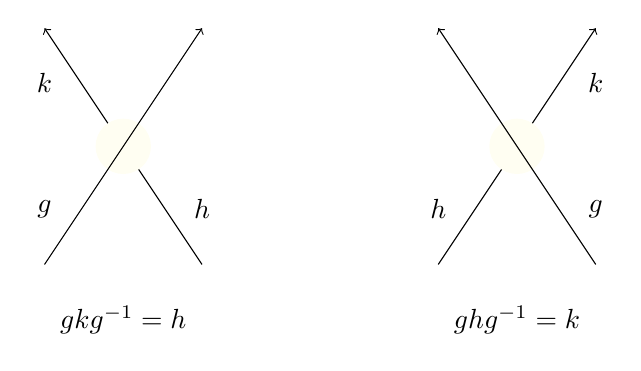
\begin{tikzpicture}
      \begin{scope}
        \draw[->] (2, 0)--(0, 3);
        \fill[yellow!5] (1, 1.5) circle (10pt);
        \draw[->] (0, 0)--(2, 3);
        \node at (0, .7) {$g$};
        \node at (0, 2.3) {$k$};
        \node at (2, .7) {$h$};

        \node at (1, -.7) {$gkg^{-1}=h$};
      \end{scope}

      \begin{scope}[shift={(5, 0)}]
        \draw[->] (0, 0)--(2, 3);
        \fill[yellow!5] (1, 1.5) circle (10pt);
        \draw[->] (2, 0)--(0, 3);
        \node at (0, .7) {$h$};
        \node at (2, 2.3) {$k$};
        \node at (2, .7) {$g$};
        
        \node at (1, -.7) {$ghg^{-1}=k$};
      \end{scope}
    \end{tikzpicture}
  \end{center}
  Presentation $\langle S\;|\;R\rangle$ described above is called the \buff{Wirtinger presentation} \cite[Chapter~6]{livingstone}.
\end{definition}

By applying the Mayer-Vietoris sequence to $S^3=K\cup_{T^2} (S^3-K)$ or noticing that every two generators are conjugate, one can conclude that the abelianization of the knot group is always $\Z$. This leads to a short exact sequence
\begin{center}
  \begin{tikzcd}
    0\arrow[r] & K_G \arrow[r] & G=\pi_1(K)\arrow[r, "ab"] & \Z=G^{ab} \arrow[r] & 0.
  \end{tikzcd}
\end{center}

%The group $K_G=\ker(ab:G\to\Z)=[G, G]$ in general is neither abelian nor finitely generated, an observation that is discussed in \cref{alexander module discussion}, and thus is a difficult group to work with. However, its abelianization $K_G^{ab}=K_G/[K_G, K_G]$ allows a $\Z[\Z]$ module structure and thus contains information about the knot $K$. 
The presentation of the group $K_G=\ker(ab:G\to\Z)=[G,G]$ obtained from a Wirtinger presentation of $G$ is discussed in \cref{alexander module discussion}.

\begin{lemma}\label{komutator komutatora jest normalny}
  For any group $G$, the commutator of its commutator $K_G$ is a normal subgroup: \hl{$[K_G, K_G]=[[G, G], [G, G]]\triangleleft G$}. 
\end{lemma}

\begin{proof}
  The commutator subgroup is a characteristic subgroup, since for any automorphism $\phi:G\to G$ 
  $$\phi(hgh^{-1}g^{-1})=\phi(h)\phi(g)\phi(h)^{-1}\phi(g)^{-1}\in K_G=[G, G].$$
  Conjugation by any element $g\in G$ is an automorphism of the commutator $K_G$. Thus it preserves its commutator subgroup $[K_G, K_G]$. 
\end{proof}

The exact sequence
\begin{equation}\label{split sequence metab}
  \begin{tikzcd}
    0\arrow[r] & K_G^{ab} \arrow[r] & G^{mab}=G/[K_G, K_G]\arrow[r] & \Z \arrow[r] & 0
  \end{tikzcd}
\end{equation}
is exact.

% If $G$ is considered in its Wirtinger presentation, then $K_G$ does not have a finite set of generators. If $a_1$,..., $a_s$ where the generators of $G$ such that $(a_i)^{ab}=1$ for every $i$, then choosing new generators to be $x_i=a_ia_1^{-1}$ for $i=2,..., s$ implies that $K$ is generated by $a_1^{k}x_ia_1^{-k}$ for $i=2,...,s$ and $k\in\Z$.

\begin{definition}[metabelianization]\label{metab def}
  The quotient group $G^{mab}=G/[K_G, K_G]$ is called the \buff{metabelianization} of $G$. 
\end{definition}

\begin{proposition}\label{dzialanie na KG}
  $$G^{mab}\cong K_G^{ab}\rtimes \Z$$
\end{proposition}

\begin{proof}
  By \cref{komutator komutatora jest normalny} we know that $[K_G, K_G]\triangleleft K_G$ are normal subgroups of $G$, then by the third isomorphism theorem, $K_G^{ab}=K_G/[K_G, K_G]$ is also a normal subgroup in $G/[K_G, K_G]$.
  The sequence \eqref{split sequence metab} is split because $\Z\to G^{mab}\to\Z$ defined by $1\mapsto a\mapsto 1$, where $a$ is any generator of $G^{mab}$ is the identity map on $\Z$. This completes the proof.
\end{proof}

\Cref{dzialanie na KG} implies that there exists an action of $\Z$ on the $\Z$-module $K_G^{ab}$. Thus, a $\Z[\Z]$-module structure is admissible on $K_G^{ab}$. 
We will return to the concept of metabelianization and $K_G^{ab}$ in \cref{section2}, specifically in \cref{alexander module discussion}. For the time being, let us assign a name to $K_G^{ab}$:

\begin{definition}[Alexander module]\label{alexander module def}
  Given a group $G$ with a homomorphism $g:G\to \Z$, the abelianization of the kernel $\ker(g)$, $K_G^{ab}$, with $\Z[\Z]$-module structure is called the \buff{Alexander module} of $G$. If $G$ is a knot group, then $\ker(g)=[G, G]=K_G$ and it is the Alexander module of the knot $K$.
\end{definition}




